\documentclass{article}
\usepackage[utf8]{inputenc} % Required for inputting international characters
\usepackage[T1]{fontenc} % Output font encoding for international characters
\usepackage{pdfpages}
\usepackage{mathpazo} % Use the Palatino font by default

%\usepackage[backend=bibtex,style=authoryear,natbib=true]{biblatex} % Use the bibtex backend with the authoryear citation style (which resembles APA)

%\addbibresource{reference_library.bib} % The filename of the bibliography

\usepackage[autostyle=true]{csquotes} % Required to generate language-dependent quotes in the bibliography

\begin{document}
\section*{I'm not hiding here because I ate the schematics, honest!}

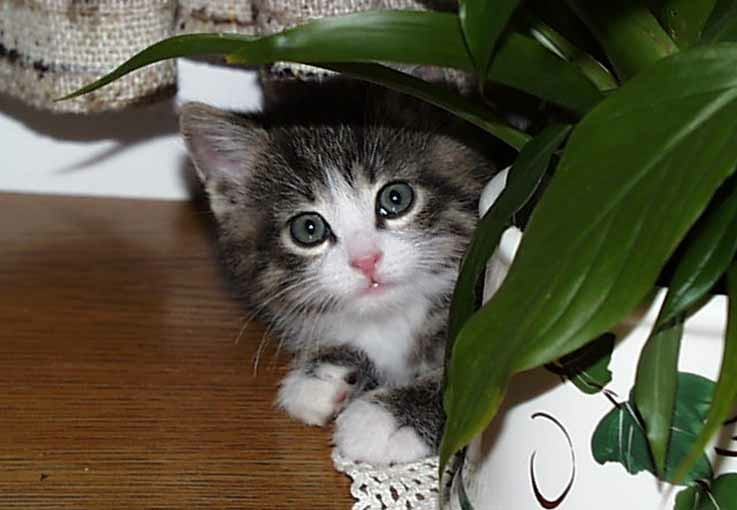
\includegraphics{kitty.png}
{Image License CC-BY-SA-3.0 https://commons.wikimedia.org/wiki/File:Young\_cat.png}
\end{document}
